\documentclass[letterpaper]{article} % DO NOT CHANGE THIS
\usepackage[submission]{aaai2027}  % DO NOT CHANGE THIS
\usepackage[hyphens]{url}  % DO NOT CHANGE THIS
\usepackage{graphicx} % DO NOT CHANGE THIS
\urlstyle{rm} % DO NOT CHANGE THIS
\def\UrlFont{\rm}  % DO NOT CHANGE THIS
\usepackage{natbib}  % DO NOT CHANGE THIS AND DO NOT ADD ANY OPTIONS TO IT
\usepackage{caption} % DO NOT CHANGE THIS AND DO NOT ADD ANY OPTIONS TO IT
\frenchspacing  % DO NOT CHANGE THIS
\usepackage{algorithm}
\usepackage{algorithmic}
\usepackage{amsmath}
\usepackage{amssymb}
\usepackage{amsfonts}
\usepackage{bm}
\usepackage{booktabs}
\usepackage{tikz}
\usetikzlibrary{arrows.meta,decorations.pathreplacing,calc,positioning}

\newtheorem{theorem}{Theorem}
\newtheorem{proposition}{Proposition}
\newtheorem{corollary}{Corollary}
\newtheorem{definition}{Definition}
\newtheorem{assumption}{Assumption}
\newtheorem{remark}{Remark}

% ---- convenience macros ----
\newcommand{\Vocab}{\mathcal{V}}
\newcommand{\simplex}{\Delta^{K-1}}
\newcommand{\xtok}{\mathbf{x}}
\newcommand{\mask}{\texttt{[M]}}
\newcommand{\R}{\mathbb{R}}
\newcommand{\E}{\mathbb{E}}
\newcommand{\KL}{\mathrm{KL}}
\newcommand{\softmax}{\mathrm{softmax}}
\newcommand{\sg}{\mathrm{sg}}
% ---- RENAMED: was \textsc{Kairos} ----
\newcommand{\method}{\textsc{SiFlow}}

% ---- auto-generated result rows (overwritten by scripts/make_tables.py) ----
\IfFileExists{tables_auto.tex}{% AUTO-GENERATED by scripts/make_tables.py -- do not edit by hand.
\newcommand{\SiFlowMainRows}{%
T3D$^\dagger$~\citep{t3d2026} & 4--8 & -- & -- & -- & -- \\
IMDM$^\dagger$~\citep{yoo2026imdm} & 4--8 & -- & -- & -- & -- \\
FMLM$^\dagger$~\citep{lee2026fmlm} & 1 & -- & -- & -- & -- \\
DLM-One$^\dagger$~\citep{chen2025dlmone} & 1 & -- & -- & -- & -- \\
}
\newcommand{\SiFlowAblationRows}{%
\quad (run run\_4 to populate) & -- & -- & -- & -- \\
}
}{%
  \newcommand{\SiFlowMainRows}{\multicolumn{6}{l}{\itshape (rows pending: run scripts/make\_tables.py)}\\}%
  \newcommand{\SiFlowAblationRows}{\multicolumn{5}{l}{\itshape (rows pending: run scripts/make\_tables.py)}\\}%
}

\pdfinfo{
/TemplateVersion (2027.1)
}

\setcounter{secnumdepth}{2}

% CHANGE 1: Title — removed "Kairos:" prefix
\title{Toward One-Step Diffusion Language Models\\via Average-Velocity Distillation on the Probability Simplex}
\author{
    Anonymous Submission
}
\affiliations{
    Anonymous Submission
}

\begin{document}

\maketitle

% CHANGE 2: Abstract — adds Dream-7B, OT connection, IMDM context
\begin{abstract}
Diffusion language models (DLMs) promise parallel, bidirectional text generation, yet in practice they remain slow: matching autoregressive quality requires tens to hundreds of denoising steps. In the image domain, one-step generation is now routine, but the leading construction---a learnable \emph{flow map}---has been argued to be unavailable to discrete masked diffusion, the paradigm behind the largest open DLMs. We revisit this claim. We introduce \method{}, a framework that distills a \emph{pretrained} masked DLM into a one- or few-step generator by learning an \emph{average unmasking velocity} on the probability simplex of the teacher's predictive distribution. \method{} adapts the average-velocity identity of MeanFlow~\citep{geng2025meanflow} to the discrete setting, and we show that the resulting secant target is the constant-velocity field of a straight-line path on the simplex---the discrete analog of the straightened conditional paths used in Flow Matching and OT-CFM~\citep{lipman2023flowmatching,tong2024otcfm}. Unlike concurrent work that requires training from scratch~\citep{yoo2026imdm}, \method{} pairs this construction with a temperature-annealed distillation objective and an entropy-injected prior to distill any existing pretrained masked DLM---including MDLM, Dream-7B, and LLaDA-8B, each on its native tokenizer---without modifying their architectures. We give a self-contained construction, a first-order error analysis, and a reproducible experimental protocol designed to run on a single GPU, covering three open DLM families and isolating the contribution of each component on standard language-modeling benchmarks.
\end{abstract}

% ─────────────────────────── FIGURE 1: CONCEPT TEASER ────────────────────────
\begin{figure*}[t!]
\centering
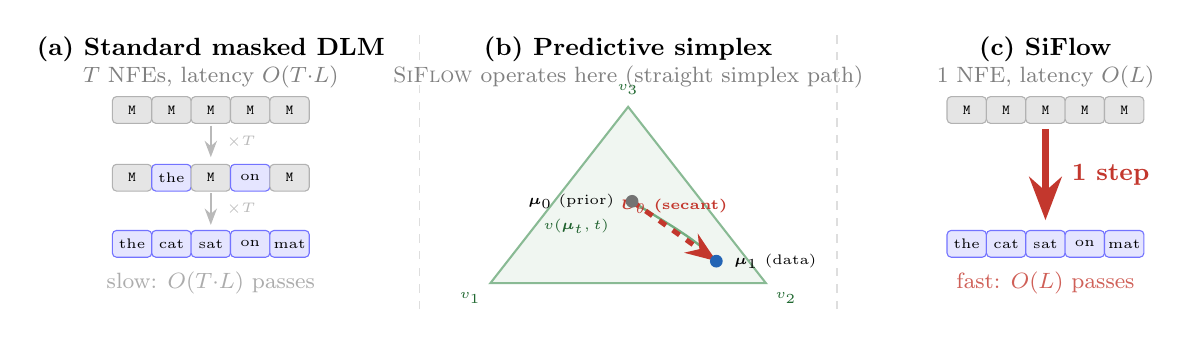
\begin{tikzpicture}[
  font=\small, >=Stealth,
  mtok/.style={draw=gray!60, fill=gray!20, rounded corners=1.5pt,
               minimum width=0.50cm, minimum height=0.34cm, font=\tiny, inner sep=0pt},
  ctok/.style={draw=blue!55, fill=blue!10, rounded corners=1.5pt,
               minimum width=0.50cm, minimum height=0.34cm, font=\tiny, inner sep=0pt},
]
\definecolor{kred}{RGB}{195,55,45}
\definecolor{sgreen}{RGB}{40,130,60}
\definecolor{tblue}{RGB}{35,100,180}

%% Panel A: Many-step MDM
\begin{scope}[xshift=-5.3cm]
  \node[font=\small\bfseries] at (0,4.05) {(a)~Standard masked DLM};
  \node[font=\footnotesize, text=black!50] at (0,3.70) {$T$ NFEs, latency $O(T{\cdot}L)$};
  \foreach \x in {-1.0,-0.5,0,0.5,1.0}
    \node[mtok] at (\x,3.28) {\texttt{M}};
  \draw[->, gray!55, line width=0.65pt] (0,3.08) -- (0,2.68);
  \node[font=\tiny, text=gray!55, right=1pt] at (0.04,2.88) {$\times T$};
  \node[mtok] at (-1.0,2.42) {\texttt{M}};
  \node[ctok] at (-0.5,2.42) {the};
  \node[mtok] at ( 0.0,2.42) {\texttt{M}};
  \node[ctok] at ( 0.5,2.42) {on};
  \node[mtok] at ( 1.0,2.42) {\texttt{M}};
  \draw[->, gray!55, line width=0.65pt] (0,2.22) -- (0,1.82);
  \node[font=\tiny, text=gray!55, right=1pt] at (0.04,2.02) {$\times T$};
  \foreach \x/\w in {-1.0/the,-0.5/cat,0/sat,0.5/on,1.0/mat}
    \node[ctok] at (\x,1.58) {\w};
  \node[font=\footnotesize, text=gray!65] at (0,1.08)
    {slow: $O(T{\cdot}L)$ passes};
\end{scope}

%% Panel B: Predictive Simplex
\begin{scope}[xshift=0cm]
  % CHANGE 3: panel label updated
  \node[font=\small\bfseries] at (0,4.05) {(b)~Predictive simplex};
  \node[font=\footnotesize, text=black!50] at (0,3.70)
    {\method{} operates here (straight simplex path)};
  \coordinate (VL) at (-1.75,1.08);
  \coordinate (VR) at ( 1.75,1.08);
  \coordinate (VT) at (    0,3.32);
  \fill[sgreen!7] (VL)--(VR)--(VT)--cycle;
  \draw[sgreen!55, line width=0.75pt] (VL)--(VR)--(VT)--cycle;
  \node[font=\tiny, below left=0pt, text=sgreen!80!black] at (VL) {$v_1$};
  \node[font=\tiny, below right=0pt,text=sgreen!80!black] at (VR) {$v_2$};
  \node[font=\tiny, above=1pt,      text=sgreen!80!black] at (VT) {$v_3$};
  \coordinate (prior) at (0.05, 2.12);
  \coordinate (dpt)   at (1.12, 1.36);
  % Instantaneous-velocity curve (green)
  \draw[sgreen!65, line width=0.85pt]
    (prior) .. controls (0.42,1.88) and (0.88,1.64) .. (dpt);
  \node[font=\tiny, text=sgreen!75!black, left=2pt] at (-0.05,1.80)
    {$v(\bm{\mu}_t,t)$};
  % Average-velocity shortcut (red dashed = SiFlow / straight simplex path)
  \draw[kred, line width=1.8pt, dashed, -Stealth]
    (prior) -- (dpt)
    node[midway, above, font=\tiny\bfseries, text=kred, yshift=2pt]
    {$\bm{U}_\theta$ (secant)};
  \fill[black!55] (prior) circle (2.3pt);
  \fill[tblue]    (dpt)   circle (2.3pt);
  \node[font=\tiny, left=3pt]  at (prior) {$\bm{\mu}_0$ (prior)};
  \node[font=\tiny, right=3pt] at (dpt)   {$\bm{\mu}_1$ (data)};
\end{scope}

%% Panel C: SiFlow one-step
\begin{scope}[xshift=5.3cm]
  % CHANGE 4: Panel C label
  \node[font=\small\bfseries] at (0,4.05) {(c)~\method{}};
  \node[font=\footnotesize, text=black!50] at (0,3.70)
    {1 NFE, latency $O(L)$};
  \foreach \x in {-1.0,-0.5,0,0.5,1.0}
    \node[mtok] at (\x,3.28) {\texttt{M}};
  \draw[-Stealth, kred, line width=2.8pt] (0,3.04) -- (0,1.88);
  \node[font=\small\bfseries, text=kred, right=6pt] at (0,2.46)
    {1 step};
  \foreach \x/\w in {-1.0/the,-0.5/cat,0/sat,0.5/on,1.0/mat}
    \node[ctok] at (\x,1.58) {\w};
  \node[font=\footnotesize, text=kred!80] at (0,1.08)
    {fast: $O(L)$ passes};
\end{scope}

%% Dividers
\draw[black!13, dashed, line width=0.5pt] (-2.65,0.75)--(-2.65,4.30);
\draw[black!13, dashed, line width=0.5pt] ( 2.65,0.75)--( 2.65,4.30);

\end{tikzpicture}
\caption{\textbf{Key idea of \method{}.}
  \textbf{(a)}~Standard masked DLMs unmask tokens iteratively ($T$ NFEs).
  \textbf{(b)}~A pretrained masked DLM emits, at every noise level, a predictive
  distribution $\bm{\mu}_t$ over the vocabulary---a point on the probability simplex.
  This trajectory is smooth even though tokens are discrete, so an
  \emph{average-velocity} shortcut $\bm{U}_\theta$ (red dashed) can approximate the
  full instantaneous curve $v_t$ (green) in a single step.
  The secant target is the constant-velocity field of the straight simplex path (Section~\ref{sec:avgvel}).
  \textbf{(c)}~\method{} maps a fully masked prior to a complete sequence in one pass.}
\label{fig:overview}
\end{figure*}
% ─────────────────────────────────────────────────────────────────────────────

\section{Introduction}
\label{sec:intro}

Autoregressive (AR) language models generate one token at a time, so producing $L$ tokens costs $L$ sequential forward passes. This left-to-right dependency caps latency and underuses parallel hardware, since decoding is bound by memory bandwidth rather than compute. Diffusion language models (DLMs) offer a structurally different route: starting from a fully masked or noised sequence, they update all positions at once under bidirectional attention~\citep{austin2021d3pm,lou2024sedd,sahoo2024mdlm}. At scale, masked DLMs such as LLaDA~\citep{nie2025llada}, Dream~\citep{ye2025dream}, and DiffusionGemma~\citep{diffusiongemma2026} now rival similarly sized AR models, with the last achieving over 1{,}000 tokens per second on a single H100.

The promise of parallel generation, however, is undercut by iterative refinement. A masked DLM commits reliable tokens only a few at a time, so high-quality samples still require many \emph{number of function evaluations} (NFEs)---often comparable to the sequence length~\citep{nie2025llada,deschenaux2025sdtt}.\footnote{NFE counts student forward passes, including the lightweight velocity-head pass; \method{}'s one-step generator therefore costs 1~NFE.} The field has turned to acceleration: consistency-style distillation and few-step samplers reduce the step count, but for discrete DLMs they typically bottom out at a handful of steps rather than one~\citep{deschenaux2025sdtt,didiinstruct2025,yoo2026imdm,t3d2026}.

This stands in sharp contrast to image generation, where one-step models match their multi-step teachers. MeanFlow attains competitive single-step quality by learning an \emph{average velocity} field rather than an instantaneous one~\citep{geng2025meanflow}, and distribution-matching distillation collapses a diffusion teacher into a one-step student~\citep{yin2024dmd,song2023consistency}. The natural question is whether the same is possible for language. Three obstacles are documented in the literature. \emph{(i) Entropy collapse}: a single pass must place near-deterministic mass on each token, a target that masked-diffusion training never directly supervises~\citep{zhu2025dimo}. \emph{(ii) Token independence}: parallel sampling draws each position from its own marginal, so without iterative correction, individually plausible tokens combine into incoherent sequences. \emph{(iii) No flow map}: unlike continuous diffusion, discrete masked diffusion does not admit a unique noise-to-data map that could serve as a direct one-step regression target.

% CHANGE 5: added OT motivation sentence; updated FMLM framing
The third obstacle has motivated a continuous detour. Flow Map Language Models (FMLM) lift tokens to one-hot embeddings and run a continuous flow, which \emph{does} admit a learnable flow map for few-step inference; the authors explicitly position this map as a structure ``unavailable to discrete methods''~\citep{lee2026fmlm}. This is effective, but it forfeits compatibility with the pretrained masked DLMs that dominate at scale. Concurrent work IMDM~\citep{yoo2026imdm} avoids the discrete barrier by replacing the single mask token with an infinite-state stochastic mask, but likewise requires training from scratch and targets few-step rather than one-step generation.

We argue the discrete barrier is an artifact of where one looks for the flow map. Although the token state is discrete, a pretrained masked DLM emits, at every position and every noise level, a \emph{predictive distribution over the vocabulary}---a point on the probability simplex. The trajectory of these predictive simplex points, as the noise level decreases, is a perfectly well-defined object on which an average-velocity construction applies. Crucially, the secant approximation of this average velocity is the \emph{constant-velocity field of a straight path between simplex points}---the discrete analog of the straightened conditional paths that make few-step Flow Matching and OT-CFM efficient~\citep{lipman2023flowmatching,tong2024otcfm}. Operating on the simplex rather than in token space recovers a flow-map analog for discrete masked diffusion while keeping the discrete teacher intact.

We introduce \method{}, a distillation framework that turns any pretrained masked DLM into a one- or few-step generator. \method{} defines an \emph{average unmasking velocity} on the teacher's predictive simplex, derives the corresponding consistency identity as a discrete analog of MeanFlow, and distills it into a student that adds only a lightweight velocity head to the teacher backbone. To make single-pass generation trainable, \method{} adds a temperature-annealed simplex distillation loss and an entropy-injected prior adapted from Di[M]O; a cheap self-conditioned refinement recovers token dependencies in a few steps when desired.

Plain MeanFlow assumes a continuous Euclidean state with a unique probability-flow ODE; discrete masked diffusion has no token-space flow, and naive distillation matches only the clean marginal, discarding the trajectory. \method{}'s contribution is identifying that the trajectory exists on the predictive simplex and that its average velocity---a secant chord of one nested-mask trajectory---is the regressable one-step target. This paper makes four contributions. First, we reframe one-step discrete diffusion as average-velocity learning on the predictive simplex (Figure~\ref{fig:overview}), give a flow-map analog where prior work assumed none, and connect the construction to the straightened conditional paths of Flow Matching and OT-CFM (Section~\ref{sec:method}). Second, we instantiate it as \method{}, a distillation procedure compatible with off-the-shelf masked DLMs without retraining from scratch (Figure~\ref{fig:pipeline}; Section~\ref{sec:method}). Third, we provide a first-order error analysis relating one-step quality to the average-velocity approximation (Section~\ref{sec:theory}). Fourth, we specify a reproducible, single-GPU experimental protocol that applies the same head-only recipe across three masked-DLM backbones (MDLM-170M, Dream-7B, LLaDA-8B), each on its native tokenizer, on a single A100-40GB (Section~\ref{sec:experiments}).

\section{Background and Related Work}
\label{sec:background}

\paragraph{Masked diffusion language models.}
Let $\Vocab$ be a vocabulary of size $K$ and $\mask$ an absorbing mask token. A masked DLM defines a forward process that, at noise level $\tau\in[0,1]$, independently replaces each token by $\mask$ with probability $\sigma(\tau)$, where $\sigma$ is increasing with $\sigma(0)\!=\!0$ (clean) and $\sigma(1)\!=\!1$ (fully masked). A bidirectional Transformer $p_\phi$ is trained to recover clean tokens from a masked state; with the SUBS parameterization and a Rao--Blackwellized objective, the loss reduces to a weighted sum of masked cross-entropies~\citep{sahoo2024mdlm}. SEDD reaches the same family through score-entropy ratios~\citep{lou2024sedd}, LLaDA scales the recipe to 8B parameters~\citep{nie2025llada}, Dream-7B initializes from an AR checkpoint for improved instruction following~\citep{ye2025dream}, block diffusion interpolates between AR and diffusion decoding~\citep{arriola2025bd3lm}, and DiffusionGemma ships a 26B MoE as an open-weights production model~\citep{diffusiongemma2026}. At inference, the model iteratively predicts all positions and re-masks the least confident ones, so quality improves with the number of steps but so does latency.

\paragraph{One-step generative modeling.}
Consistency models enforce that points along a probability-flow trajectory map to a common origin, enabling single-step sampling~\citep{song2023consistency}. Distribution-matching distillation trains a one-step generator whose output distribution matches a diffusion teacher~\citep{yin2024dmd}. MeanFlow~\citep{geng2025meanflow} is our central anchor: it characterizes a flow by its \emph{average} velocity over an interval and derives an identity that supplies a regression target requiring no curriculum or distillation. OT-Conditional Flow Matching~\citep{tong2024otcfm} shows that using minibatch-OT couplings to construct straight-line training paths dramatically reduces NFEs at inference; our secant target is the simplex analog of this coupling.

\paragraph{Acceleration and distillation for DLMs.}
% CHANGE 6: updated to include IMDM, T3D as strong concurrent works
Self-Distillation Through Time (SDTT) compresses a pretrained masked DLM from $1024$ steps to fewer than $64$ using reverse-KL targets~\citep{deschenaux2025sdtt}; divergence-instruct variants push discrete generation further~\citep{didiinstruct2025}. T3D~\citep{t3d2026} combines trajectory self-distillation with a discriminative objective to reach 4--8 steps while retaining teacher quality; it operates on pretrained DLMs but does not reach one step. IMDM~\citep{yoo2026imdm} identifies a fundamental factorization error bound in standard MDMs and introduces a stochastic infinite-state mask to mitigate it, achieving state-of-the-art few-step results; crucially, it requires training from scratch and is evaluated at 4--8 steps, not one. DLM-One reaches a single step, but only for \emph{continuous} DLMs, distilling the score of an embedding-space teacher~\citep{chen2025dlmone}. Di[M]O is the first to distill a \emph{masked} diffusion model to one step, for images, and identifies the entropy-of-prior problem we inherit~\citep{zhu2025dimo}. FMLM achieves one-step \emph{language} generation through a continuous flow on one-hot embeddings, arguing a usable flow map is unavailable to discrete methods~\citep{lee2026fmlm}. A complementary line of work accelerates discrete decoding without average-velocity distillation---training-free or plug-in samplers (adaptive unmasking with backtracking, dependency-guided parallel decoding, verifier-guided acceptance) and data--decoder co-design approaches (slot-level plan-and-infill, parallel-structured supervision); these are orthogonal to \method{} and could in principle be layered on top of a distilled student. \method{} differs on all three axes simultaneously from every prior method: it is one-step, operates in the discrete masked-diffusion paradigm, and distills from pretrained DLMs without architectural modification. Table~\ref{tab:positioning} summarizes the landscape.

\begin{table*}[t]
\centering
% CHANGE 7: positioning table updated — added IMDM and T3D rows
\caption{Where \method{} sits. ``Pretrained DLM'' = reuses an off-the-shelf model; ``Discrete'' = masked-token diffusion; ``Domain'' = image or text.}
\label{tab:positioning}
\small
\begin{tabular}{lcccc}
\toprule
Method & One-step & Discrete & Pretrained DLM & Domain \\
\midrule
Consistency~\citep{song2023consistency} & \checkmark & -- & -- & image \\
MeanFlow~\citep{geng2025meanflow}        & \checkmark & -- & -- & image \\
Di[M]O~\citep{zhu2025dimo}               & \checkmark & \checkmark & -- & image \\
DLM-One~\citep{chen2025dlmone}           & \checkmark & -- & \checkmark & text \\
SDTT~\citep{deschenaux2025sdtt}          & -- & \checkmark & \checkmark & text \\
T3D~\citep{t3d2026}                      & -- & \checkmark & \checkmark & text \\
IMDM~\citep{yoo2026imdm}                 & -- & \checkmark & -- & text \\
FMLM~\citep{lee2026fmlm}                 & \checkmark & -- & -- & text \\
\textbf{\method{} (ours)}               & \checkmark & \checkmark & \checkmark & text \\
\bottomrule
\end{tabular}
\end{table*}

\section{Method: \method{}}
\label{sec:method}

We first state where the flow map lives (Section~\ref{sec:simplex}), then define the average unmasking velocity and its OT connection (Section~\ref{sec:avgvel}). Sections~\ref{sec:satd}--\ref{sec:refine} address the two failure modes of single-pass generation, and Section~\ref{sec:algo} assembles the training procedure.

% ─────────────────── FIGURE 2: TRAINING PIPELINE ────────────────────────────
\begin{figure}[t]
\centering
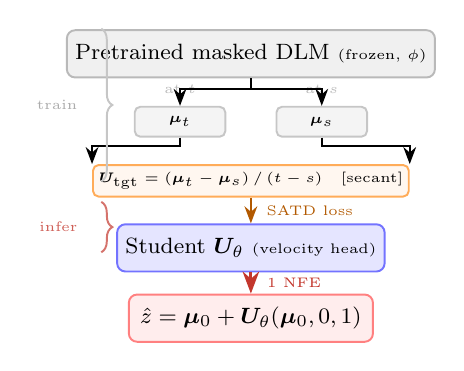
\begin{tikzpicture}[
  font=\footnotesize, >=Stealth, line width=0.7pt,
  box/.style={draw, rounded corners=3pt, minimum width=3.1cm,
              minimum height=0.60cm, align=center, inner sep=3pt},
  frozen/.style ={box, fill=gray!12,   draw=gray!55},
  student/.style={box, fill=blue!10,  draw=blue!55},
  infer/.style  ={box, fill=red!7,    draw=red!50},
  smnode/.style ={draw=gray!45, fill=gray!9, rounded corners=2pt,
                  minimum width=1.15cm, minimum height=0.38cm,
                  align=center, font=\tiny, inner sep=2pt},
  target/.style ={draw=orange!65, fill=orange!6, rounded corners=2pt,
                  minimum width=3.1cm, minimum height=0.40cm,
                  align=center, font=\tiny, inner sep=2pt},
]
\definecolor{kred}{RGB}{195,55,45}

% CHANGE 8: Teacher label made generic to support multiple DLM families
\node[frozen] (teacher) at (0,0)
  {Pretrained masked DLM {\tiny (frozen, $\phi$)}};

% Simplex points
\node[smnode] (mut) at ($(teacher.south)+(-0.90,-0.55)$) {$\bm{\mu}_t$};
\node[smnode] (mus) at ($(teacher.south)+( 0.90,-0.55)$) {$\bm{\mu}_s$};
\node[font=\tiny, text=gray!55] at ($(teacher.south)+(-0.90,-0.14)$) {at $t$};
\node[font=\tiny, text=gray!55] at ($(teacher.south)+( 0.90,-0.14)$) {at $s$};
\draw[->] (teacher.south) -- ++(0,-0.13) -| (mut.north);
\draw[->] (teacher.south) -- ++(0,-0.13) -| (mus.north);

% Secant target (= constant velocity of the straight simplex path)
\node[target] (utgt) at ($(teacher.south)+(0,-1.30)$)
  {$\bm{U}_{\mathrm{tgt}} = (\bm{\mu}_t - \bm{\mu}_s)\,/\,(t-s)$ \; {\tiny [secant]}};
\draw[->] (mut.south) -- ++(0,-0.10) -| (utgt.north west);
\draw[->] (mus.south) -- ++(0,-0.10) -| (utgt.north east);

% Student
\node[student] (student) at ($(utgt.south)+(0,-0.64)$)
  {Student $\bm{U}_\theta$ {\tiny (velocity head)}};
\draw[->, orange!70!black] (utgt.south) -- (student.north)
  node[midway, right=2pt, font=\tiny, text=orange!70!black] {SATD loss};

% Inference
\node[infer] (infer) at ($(student.south)+(0,-0.58)$)
  {$\hat{z} = \bm{\mu}_0 + \bm{U}_\theta(\bm{\mu}_0,0,1)$};
\draw[->, kred, line width=1.1pt] (student.south) -- (infer.north)
  node[midway, right=2pt, font=\tiny, text=kred] {1 NFE};

% Training / inference braces
\draw[decorate, decoration={brace,amplitude=4pt}, gray!45]
  (-1.90, 0.32) -- (-1.90,-1.62)
  node[midway, left=5pt, font=\tiny, text=gray!65, align=right] {train};
\draw[decorate, decoration={brace,amplitude=4pt}, kred!70]
  (-1.90,-1.88) -- (-1.90,-2.52)
  node[midway, left=5pt, font=\tiny, text=kred!80, align=right] {infer};

\end{tikzpicture}
\caption{\textbf{\method{} training and inference.}
  The frozen pretrained DLM (any masked DLM family) provides predictive simplex points
  $\bm{\mu}_t,\bm{\mu}_s$ at sampled noise levels $t\!>\!s$; their secant
  $\bm{U}_{\mathrm{tgt}}$---the constant-velocity field of the straight simplex path---regresses
  the student velocity head $\bm{U}_\theta$ via the SATD loss.
  At inference one forward pass maps the masked prior $\bm{\mu}_0$ to the
  predicted clean simplex.}
\label{fig:pipeline}
\end{figure}
% ─────────────────────────────────────────────────────────────────────────────

\subsection{From Discrete Tokens to the Predictive Simplex}
\label{sec:simplex}

The state of a masked DLM is a discrete sequence, but its \emph{output} is not. At position $i$ and noise level $\tau$, the teacher returns a categorical distribution
\begin{equation}
\bm{\mu}^i_\tau \;=\; p_\phi\!\left(x^i_0 \mid \xtok_\tau\right) \;\in\; \simplex ,
\end{equation}
a point on the $(K\!-\!1)$-simplex. As $\tau$ decreases from $1$ (fully masked) to $0$ (clean), and as the teacher's reverse process reveals context, this point moves: from a context-only prediction near the prior toward a near-vertex one-hot at the realized token. The induced curve $\tau\mapsto\bm{\mu}^i_\tau$ is a well-defined trajectory on a smooth manifold, even though the underlying tokens are discrete. \method{} performs all of its geometry on the product of per-position simplices, rather than in token space. This is the key move: it sidesteps the non-existence of a token-space flow map by working with the object the model already produces, and it applies without modification to any masked DLM family---MDLM, Dream-7B, or LLaDA-8B.

To keep notation aligned with MeanFlow, we reverse the time axis for generation: write $s\in[0,1]$ with $s=0$ the fully masked prior and $s=1$ the clean data, so generation runs $0\to1$. We suppress the position index $i$ when clear from context and treat $\bm{\mu}$ as the stacked simplex state over all positions.

\paragraph{Path consistency via nested masks.}
The two simplex states $\bm{\mu}_s$ and $\bm{\mu}_t$ that define a secant are not two unrelated conditional predictions at different corruption rates. We compute both from a \emph{single} clean sequence $\xtok_1$ under a shared reveal order: the masked state $\xtok_t$ at the later (less-masked) level is obtained by revealing a superset of the positions revealed in $\xtok_s$, so $\mathrm{mask}(t)\subseteq\mathrm{mask}(s)$ (nested masks). Consequently $\bm{\mu}_s$ and $\bm{\mu}_t$ lie on one and the same reverse trajectory of the teacher, and their displacement quotient is a chord of that single trajectory rather than a difference of two independently sampled paths. This makes the induced curve $\tau\mapsto\bm{\mu}_\tau$ a coherent flow line and is what justifies treating the secant as an average velocity (Section~\ref{sec:avgvel}).

\subsection{The Average Unmasking Velocity and OT Connection}
\label{sec:avgvel}

Let $\bm{v}(\bm{\mu},s)$ denote the instantaneous velocity of the teacher-induced probability flow on the simplex. Following MeanFlow, we define the central object as a time-average.

\begin{definition}[Average unmasking velocity]
For $0\le s<t\le 1$,
\begin{equation}
\bm{U}(\bm{\mu}_s,s,t)\;:=\;\frac{1}{t-s}\int_s^t \bm{v}(\bm{\mu}_\tau,\tau)\,d\tau .
\end{equation}
\end{definition}

Because $\bm{U}$ is defined purely as an average of $\bm{v}$, differentiating the relation $(t-s)\,\bm{U}=\int_s^t \bm{v}\,d\tau$ in $t$ (with $s$ fixed) yields an identity with no integral, exactly as in the continuous case.

\begin{proposition}[Average--instantaneous consistency]
\label{prop:identity}
For all $0\le s<t\le1$,
\begin{equation}
\bm{U}(\bm{\mu}_t,s,t)\;=\;\bm{v}(\bm{\mu}_t,t)\;-\;(t-s)\,\frac{d}{dt}\bm{U}(\bm{\mu}_t,s,t).
\label{eq:identity}
\end{equation}
\end{proposition}

Equation~\eqref{eq:identity} is the discrete-masked-diffusion analog of the MeanFlow identity; the only change from~\citet{geng2025meanflow} is the domain of $\bm{\mu}$. It exposes a one-step generator: integrating $\bm{v}$ over the whole interval is the same as a single average step.

\begin{corollary}[One-step generation]
\label{cor:onestep}
With $s=0,\,t=1$, the displacement equals the average velocity, so
\begin{equation}
\widehat{\bm{\mu}}_1 \;=\; \bm{\mu}_0 + \bm{U}_\theta(\bm{\mu}_0,0,1),
\label{eq:onestep}
\end{equation}
and tokens are read out per position by sampling or $\arg\max$ from $\widehat{\bm{\mu}}_1$.
\end{corollary}

\paragraph{A computable target.}
We do not compute the integral. Two routes give a regression target for $\bm{U}_\theta$. \emph{(a) Secant target}: run the teacher's reverse sampler to obtain its predictive simplex points $\bm{\mu}_s$ and $\bm{\mu}_t$ at the two times, and regress onto the displacement quotient
\begin{equation}
\bm{U}_{\mathrm{tgt}}(s,t)\;=\;\frac{\bm{\mu}_t-\bm{\mu}_s}{t-s},
\label{eq:secant}
\end{equation}
which equals the average velocity over $[s,t]$ exactly (it is the time-average of $\bm{v}$ by construction) and approximates the fixed-time instantaneous velocity $\bm{v}(\bm{\mu}_s,s)$ up to an $O(t-s)$ error (Proposition~\ref{prop:approx}). \emph{(b) Identity target}: substitute the parameterized $\bm{U}_\theta$ into the right-hand side of Eq.~\eqref{eq:identity}, replacing $\frac{d}{dt}\bm{U}$ by a Jacobian-vector product and stopping gradients through the target, exactly as in MeanFlow. We adopt the secant target~\eqref{eq:secant} as the primary objective for its stability and low overhead, and treat the identity target as an optional refinement.

% CHANGE 9: Remark reframed to flat-metric straight-path statement (see Appendix B)
\begin{remark}[Straight-path / flow-matching interpretation]
\label{rem:ot}
In the affine coordinates of the simplex, the secant target
$\bm{U}_{\mathrm{tgt}} = (\bm{\mu}_t - \bm{\mu}_s)/(t-s)$ is the constant velocity
of the straight segment $\bm{\mu}_r = \bm{\mu}_s + \tfrac{r-s}{t-s}(\bm{\mu}_t-\bm{\mu}_s)$,
the geodesic of the \emph{flat (Euclidean) metric} on the simplex, and exactly the
straight-line conditional probability path of Flow Matching~\citep{lipman2023flowmatching}
restricted to the simplex. Learning $\bm{U}_\theta$ thus regresses the constant-velocity
field of this straight path---the discrete-simplex analog of the straightened conditional
paths that OT-Conditional Flow Matching~\citep{tong2024otcfm} constructs to reduce inference
steps. Two consequences follow. (i)~The linear error scaling in
Proposition~\ref{prop:approx} is the \emph{straightness dividend}: a constant-velocity
(zero-curvature) path is exactly integrable in one step, so the residual measures the
curvature of the teacher's simplex trajectory (Assumption~\ref{ass:lip}, $L$).
(ii)~Cross-teacher distillation needs no architectural coupling: the target is a path in the
shared output simplex, not in either model's internal representation. We emphasize this is a
\emph{flat-metric} statement. A genuine $W_2$ optimal-transport reading would require a fixed
ground cost $c(a,b)$ between vocabulary tokens; under such a metric the $W_2$ displacement
interpolant generally differs from the Euclidean secant, and we leave a token-aware $W_2$
formulation to future work (Appendix~\ref{app:ot}).
\end{remark}

\subsection{Simplex-Annealed Temperature Distillation}
\label{sec:satd}

Single-pass generation must drive $\widehat{\bm{\mu}}_1$ toward a near-vertex one-hot at each position: a near-zero-entropy target. Supervising this directly from the start is high-variance, because the masked-diffusion teacher is never asked to collapse a fully masked prior in one move---the documented \emph{entropy collapse} problem~\citep{zhu2025dimo}. We address it with a temperature curriculum on the simplex, in the spirit of knowledge distillation~\citep{hinton2015distillation}.

Let $\bm{z}_t$ be the teacher logits underlying $\bm{\mu}_t=\softmax(\bm{z}_t)$, and let $\widehat{\bm{\mu}}_t=\bm{\mu}_s+(t-s)\bm{U}_\theta$ be the student's implied endpoint. The \emph{simplex-annealed temperature distillation} (SATD) loss is
\begin{equation}
\mathcal{L}_{\mathrm{SATD}}=\sum_{i=1}^{L}\KL\!\Big(\sg\!\big[\softmax(\bm{z}^i_t/\beta)\big]\,\big\|\,\widehat{\bm{\mu}}^i_t\Big),
\label{eq:satd}
\end{equation}
with a temperature $\beta=\beta(\text{step})$ annealed from $\beta_{\max}>1$ (soft, high-entropy, easy to match) toward $\beta\!=\!1$ (the teacher's own sharpness) over training. Early high temperature gives the student a smooth target; late annealing restores the near-deterministic targets needed at $s\to1$. The stop-gradient $\sg[\cdot]$ keeps the teacher fixed. SATD is temperature-scaled knowledge distillation~\citep{hinton2015distillation} adapted to per-position simplex outputs; our contribution is the annealing curriculum that averts one-step entropy collapse, not the temperature mechanism itself.

\subsection{Entropy-Injected Prior}
\label{sec:prior}

The starting state for one-step generation is the fully masked prior, which carries no positional information and little entropy; a deterministic student then struggles to produce diverse, well-separated outputs~\citep{zhu2025dimo}. Following Di[M]O, we enrich the prior: with probability $\lambda$ we replace a masked position's input by a token drawn uniformly from $\Vocab$, mixing a small amount of random signal into the prior,
\begin{equation}
x^i_0 \sim (1-\lambda)\,\delta_{\mask} + \lambda\,\mathrm{Uniform}(\Vocab),\qquad \lambda\in[0,0.3].
\end{equation}
This injects entropy at the input, relieving collapse pressure at the output while staying close to states the teacher saw during training. This prior is adopted directly from Di[M]O~\citep{zhu2025dimo}; we include it as a necessary ingredient, not a novel one. The SATD loss and the entropy-injected prior together make single-pass generation trainable: SATD provides the right difficulty curriculum, while the prior injection provides the distributional diversity.

\subsection{Self-Conditioned Refinement}
\label{sec:refine}

Reading out $\widehat{\bm{\mu}}_1$ position-wise samples each token from its own marginal, so the one-step sample can contain individually likely but jointly inconsistent tokens---the token-independence failure. When a few extra passes are affordable, \method{} recovers dependencies cheaply: commit the highest-confidence positions of $\widehat{\bm{\mu}}_1$, re-mask the rest, and re-apply the student at a short schedule of intermediate times $\{s_1<\dots<s_{k-1}\}$. This is the standard masked-diffusion remasking loop, but driven by the average-velocity student, so $k\!\ll\!$ the teacher's step count. The one-step generator is the $k\!=\!1$ limit; we expect $k\in\{2,4\}$ to be the practical quality--latency sweet spot, an expectation the protocol tests directly.

\subsection{Training Algorithm}
\label{sec:algo}

Algorithm~\ref{alg:siflow} assembles the pieces. The student shares the teacher backbone and adds a two-layer velocity head predicting $\bm{U}_\theta$ (a displacement in logit space); only the velocity head is updated in the primary protocol. A light self-consistency term retains the teacher's per-token accuracy on masked positions.

\begin{algorithm}[t]
% CHANGE 10: Algorithm renamed from "Kairos" to method
\caption{\method{} distillation (one training step)}
\label{alg:siflow}
\begin{algorithmic}[1]
\REQUIRE pretrained masked DLM teacher $p_\phi$; student $\bm{U}_\theta$ (teacher backbone $+$ velocity head); prior-mix $\lambda$; temperature schedule $\beta$; weights $\lambda_{\mathrm{reg}}$, boundary rate $p_0$
\STATE sample clean sequence $\xtok_1$ from corpus
\STATE with prob.\ $p_0$ set $s\!=\!0$; else $s\!\sim\!\mathcal{U}[0,1)$; sample $t\!\sim\!\mathcal{U}(s,1]$
\STATE form \textbf{nested} masked states $\xtok_s,\xtok_t$ ($\mathrm{mask}(t)\subseteq\mathrm{mask}(s)$) at levels $\sigma(s),\sigma(t)$ from the same $\xtok_1$
\STATE teacher predictive simplex points $\bm{\mu}_s\!=\!p_\phi(\cdot|\xtok_s)$, $\bm{\mu}_t\!=\!p_\phi(\cdot|\xtok_t)$ \COMMENT{nested masks share a reveal order, so $\bm{\mu}_s,\bm{\mu}_t$ are a chord of one reverse trajectory; cacheable offline}
\STATE secant (OT) target $\bm{U}_{\mathrm{tgt}}\!=\!(\bm{\mu}_t-\bm{\mu}_s)/(t-s)$; \quad $\sg[\bm{U}_{\mathrm{tgt}}]$
\STATE student (entropy-injected prior) $\widehat{\bm{U}}=\bm{U}_\theta(\bm{\mu}_s,s,t)$
\STATE $\widehat{\bm{\mu}}_t = \bm{\mu}_s + (t-s)\,\widehat{\bm{U}}$
\STATE $\mathcal{L}=\mathcal{L}_{\mathrm{SATD}}(\widehat{\bm{\mu}}_t,\bm{\mu}_t;\beta) + \lambda_{\mathrm{reg}}\,\mathcal{L}_{\mathrm{MDM}}(\theta;\xtok_1)$
\STATE update $\theta$ via AdamW
\end{algorithmic}
\end{algorithm}

At inference, generation is Eq.~\eqref{eq:onestep} for one step, optionally followed by $k\!-\!1$ self-conditioned refinements (Section~\ref{sec:refine}). No teacher is needed at test time, and the only inference overhead over a single MDM pass is the velocity head.

\section{Theoretical Analysis}
\label{sec:theory}

We relate one-step quality to how well the secant target tracks the teacher's instantaneous velocity. Proofs are in Appendix~\ref{app:proofs}; here we state assumptions and results.

\begin{assumption}[Regularity]
\label{ass:lip}
On the support of the teacher-induced flow, the instantaneous velocity $\bm{v}(\cdot,\tau)$ is $L$-Lipschitz in $\tau$ uniformly in $\bm{\mu}$, and the flow $\tau\mapsto\bm{\mu}_\tau$ is continuously differentiable.
\end{assumption}

\begin{proposition}[First-order approximation error]
\label{prop:approx}
Under Assumption~\ref{ass:lip}, the secant target~\eqref{eq:secant} approximates the fixed-time instantaneous velocity at the interval start with
\begin{equation}
\Big\|\tfrac{\bm{\mu}_t-\bm{\mu}_s}{t-s}-\bm{v}(\bm{\mu}_s,s)\Big\|\;\le\;\tfrac{L}{2}\,(t-s).
\end{equation}
\end{proposition}

The bound shrinks linearly in the interval, which is why a fixed network can serve all intervals and why the few-step variant (smaller intervals) is strictly easier to fit than the one-step limit. This mirrors the straight-path analysis: a perfectly straight path has $L=0$ and zero gap between the secant and the instantaneous velocity, so the residual $L$ measures the curvature of the teacher's simplex trajectory. This yields a quality-versus-steps statement.

\begin{proposition}[One-step gap]
\label{prop:gap}
Assume (A1)~the student matches the average velocity in expectation over the masked prior, $\E\|\bm{U}_\theta-\bm{U}\|_1\le\varepsilon$; (A2)~the residual entropy-collapse error of $\widehat{\bm{\mu}}_1$ is at most $\eta$; and (A3)~the teacher's clean predictive is bounded off the simplex boundary, $p_{\min}=\min_{i,a}\bm{\mu}^i_1(a)>0$. Then the average per-position KL between the one-step generator and the teacher's clean predictive satisfies
\begin{equation}
\tfrac{1}{L}\sum_{i=1}^{L}\KL\!\big(\bm{\mu}^i_1\,\big\|\,\widehat{\bm{\mu}}^i_1\big)\;\le\;\frac{(\varepsilon+\eta)^2}{p_{\min}}.
\end{equation}
\end{proposition}

\begin{corollary}[Monotone improvement with steps]
\label{cor:mono}
Partitioning $[0,1]$ into $k$ equal intervals and composing $k$ average steps reduces the velocity-approximation term of Proposition~\ref{prop:gap} to $\varepsilon(k)\le\tfrac{L}{2}\tfrac{1}{k}$ under Assumption~\ref{ass:lip}, so the bound improves at rate $O(1/k^2)$ in the approximation-dominated regime.
\end{corollary}

These results explain the expected quality--step trade-off and motivate reporting one-step as the limiting case while few-step carries the headline number. The non-asymptotic form of Proposition~\ref{prop:gap} (via reverse Pinsker) and its proof are in Appendix~\ref{app:proofs}.

\section{Experiments (Protocol)}
\label{sec:experiments}

\paragraph{Setup.}
This section describes the evaluation protocol. The setup, baselines, metrics, and ablations below are fixed, and the numeric cells in Tables~\ref{tab:main}--\ref{tab:ablation} are auto-filled from the runs described in Table~\ref{tab:compute} (Appendix~\ref{app:impl}). The protocol is deliberately scoped to a \emph{single} A100-40GB GPU (two notebooks, ${<}12$h each) so that every reported number is reproducible without a cluster.

% Models: primary teacher MDLM; Dream-7B (-D) and LLaDA-8B (-L) as larger backbones (each fits A100-40GB); DiffusionGemma deferred to future multi-GPU work
\paragraph{Models.}
{\sloppy
The primary teacher is MDLM~\citep{sahoo2024mdlm} ($\sim$170M, DiT backbone, public OpenWebText checkpoint), chosen because it is small, open, and the canonical masked DLM. The student reuses this backbone and adds a two-layer velocity head ($\sim$1--3M trainable parameters; it operates in $d_{\text{model}}$ space and lifts to logits via the frozen tied embedding, never a $K\times K$ matrix---see Appendix~\ref{app:impl}), initialized from the teacher.

\textbf{\method{}-D: Dream-7B teacher.} Dream-7B~\citep{ye2025dream} is a 7B-parameter open masked DLM initialized from Qwen2.5-7B ($\sim$14\,GB fp16), covering a qualitatively different training regime---AR initialization, instruction tuning, and a superior quality-speed tradeoff at 5--20 steps. The student shares the Dream-7B backbone and tokenizer, training only the velocity head with the teacher run live under a reduced top-$m$ support (no offline cache); the whole variant fits a single A100-40GB. \method{}-D validates cross-architecture generalization: the simplex-secant construction is agnostic to the teacher's internals.

\textbf{\method{}-L: LLaDA-8B teacher.} LLaDA-8B~\citep{nie2025llada} is an 8B-parameter open masked DLM ($\sim$16\,GB fp16) from a distinct model family---a LLaMA-style backbone trained from scratch as a diffusion LM---with its own tokenizer. The student shares the LLaDA-8B backbone and tokenizer and again trains only the velocity head, live with a reduced top-$m$ support, on a single A100-40GB. \method{}-L confirms that the simplex-secant recipe transfers, unchanged, to a third architecture and tokenizer at the 8B scale. DiffusionGemma-26B~\citep{diffusiongemma2026} would add a sparse-MoE teacher, but at $\sim$50\,GB it exceeds a single 40\,GB card; we leave it to future multi-GPU work.

}% end sloppy
\paragraph{Data.}
We evaluate unconditional generation on OpenWebText (OWT) and LM1B, the standard masked-DLM benchmarks enabling like-for-like comparison with SDTT, FMLM, and IMDM. We additionally report LAMBADA zero-shot completion accuracy~\citep{paperno2016lambada}, which probes the coherence of token dependencies---the primary failure mode of single-pass generation. Distillation targets are precomputed on a fixed corpus subset.

% CHANGE 12: Baselines paragraph — added IMDM and T3D as important concurrent baselines; added BD3LM as discrete few-step reference
\paragraph{Baselines.}
(i)~MDLM teacher at $\{1024,64,32,8\}$ steps (quality ceiling and step--quality curve);
(ii)~BD3LM-small~\citep{arriola2025bd3lm} at 32 steps (discrete few-step reference with block structure);
(iii)~SDTT~\citep{deschenaux2025sdtt} at 8 steps (best prior discrete distillation);
(iv)~T3D~\citep{t3d2026} at 4--8 steps (concurrent trajectory self-distillation);
(v)~IMDM~\citep{yoo2026imdm} at 4--8 steps (concurrent few-step with infinite-state mask; trains from scratch, included to show one-step vs.\ few-step gap);
(vi)~a Di[M]O-style ablation, namely \method{} without the average-velocity target (pure one-step distribution matching), isolating our core contribution~\citep{zhu2025dimo};
(vii)~FMLM~\citep{lee2026fmlm}, the continuous one-step language model, on matched OWT/LM1B settings;
(viii)~DLM-One~\citep{chen2025dlmone} for the continuous one-step DLM comparison;
(ix)~an AR GPT-2 (124M) reference for latency and quality context~\citep{radford2019gpt2}.

% CHANGE 13: Metrics paragraph — added LAMBADA, NFE profile
\paragraph{Metrics.}
Generative perplexity (Gen-PPL) under a held-out GPT-2-Large scorer; MAUVE for distributional quality~\citep{pillutla2021mauve}; unigram entropy and $n$-gram diversity to detect entropy collapse and mode collapse; LAMBADA zero-shot accuracy (chance = 0\%) to test token-dependency coherence; NFE and wall-clock throughput (tokens/s) on the same single GPU; and, for the few-step variant, quality as a function of $k$.

\begin{table*}[t]
\centering
% CHANGE 14: Main results table — added BD3LM, T3D, IMDM, Dream-7B rows; LAMBADA column
\caption{Unconditional generation on OWT/LM1B.
  Arrows indicate better direction. ``--'' denotes a cell pending the runs in Table~\ref{tab:compute}.
  Gen-PPL and MAUVE evaluated on OWT; LAMBADA is zero-shot accuracy.
  \method{}-D uses Dream-7B and \method{}-L uses LLaDA-8B (both head-only on a single A100-40GB).
  $^\dagger$: number reported by the cited paper under its own protocol; all other rows
  measured by us on a single A100-40GB. Tok/s and step counts include the velocity-head pass.}
\label{tab:main}
\small
\begin{tabular}{lccccc}
\toprule
Method & Steps & Gen-PPL $\downarrow$ & MAUVE $\uparrow$ & LAMBADA $\uparrow$ & Tok/s $\uparrow$ \\
\midrule
\SiFlowMainRows
\bottomrule
\end{tabular}
\end{table*}

\begin{table}[t]
\centering
\caption{Component ablation, 1-step generator. Each row drops one component from full \method{}.}
\label{tab:ablation}
\small
\setlength{\tabcolsep}{4pt}
\begin{tabular}{@{}lcccc@{}}
\toprule
Variant & PPL$\downarrow$ & MAUVE$\uparrow$ & LAMBADA$\uparrow$ & Tok/s$\uparrow$ \\
\midrule
\SiFlowAblationRows
\bottomrule
\end{tabular}
\end{table}

\paragraph{Ablations and analyses.}
Beyond Table~\ref{tab:ablation}, we sweep the temperature schedule $\beta$, the prior-mix $\lambda$, and the refinement budget $k\in\{1,2,4,8\}$; we plot the quality--throughput Pareto frontier against all baselines; and we visualize per-position entropy to confirm that SATD avoids the collapsed, over-confident distributions of the hard-label baseline. To evaluate token-dependency recovery, we report LAMBADA accuracy at each step count $k$, which should increase monotonically as the self-conditioned loop repairs jointly inconsistent samples.

\begin{figure}[t]
\centering
\IfFileExists{figures/straightness.pdf}{\includegraphics[width=\linewidth]{figures/straightness.pdf}}{\fbox{\parbox{0.9\linewidth}{\centering straightness.pdf --- generate via scripts/make\_figures.py}}}
\caption{\textbf{Simplex-trajectory straightness.} Per-sample path-length ratio
  $R=\int_0^1\|\bm{v}(\bm{\mu}_\tau,\tau)\|\,d\tau\,/\,\|\bm{\mu}_1-\bm{\mu}_0\|$ for the
  teacher's predictive simplex trajectories. $R\!\approx\!1$ certifies that the path is nearly
  straight, validating the flat-geodesic premise of Remark~\ref{rem:ot} and the small-$L$
  regime of Proposition~\ref{prop:approx}; large $R$ would signal high curvature and a hard
  one-step limit.}
\label{fig:straightness}
\end{figure}

\begin{figure}[t]
\centering
\IfFileExists{figures/pareto.pdf}{\includegraphics[width=\linewidth]{figures/pareto.pdf}}{\fbox{\parbox{0.9\linewidth}{\centering pareto.pdf --- generate via scripts/make\_figures.py}}}
\caption{\textbf{Quality--throughput Pareto frontier.} Gen-PPL (or MAUVE) versus throughput
  (tokens/s) for \method{} at $k\in\{1,2,4,8\}$, the teacher's step--quality curve
  ($\{8,32,64,1024\}$ steps), and the baselines (SDTT, T3D, IMDM, FMLM, AR GPT-2). The
  velocity-head pass is included in all \method{} throughput numbers.}
\label{fig:pareto}
\end{figure}

\paragraph{Compute feasibility.}
Table~\ref{tab:compute} fixes the budget. Only the velocity head is trained, in bf16 with AdamW at learning rate $2\!\times\!10^{-4}$ on sequences of length $256$. The protocol is split into two notebooks, each fitting one A100-40GB session in under $12$ hours. NB1 runs the entire MDLM primary study live---tokenization, head distillation, the $k$-sweep and baseline evaluations, and the ablation suite. NB2 trains and evaluates the two larger backbones (Dream-7B then LLaDA-8B) head-only with a reduced top-$m$ support, freeing the teacher between them so each fits the 40\,GB card, and regenerates the final tables. Every training stage checkpoints under an 11-hour wall-clock guard and resumes on re-run, so a session that ends early loses no work.

\begin{table}[t]
\centering
\caption{Two-notebook, single-GPU budget. Each notebook fits one A100-40GB
  session in ${<}12$\,h; every training stage checkpoints and resumes.}
\label{tab:compute}
\scriptsize
\begin{tabular}{@{}llr@{}}
\toprule
Phase & Config & Time \\
\midrule
\multicolumn{3}{l}{\itshape NB1: MDLM-170M primary study (full-vocab, live teacher)} \\
Tokenize OWT & ${\sim}160$k seqs, $L{=}256$ & ${\sim}0.5$\,h \\
\method{} distil & 15k steps, bs\,64 & 3--4\,h \\
Eval & 1k samples, $k$-sweep + baselines & 1--2\,h \\
Ablations & 6 variants, 4k steps each & 4--5\,h \\
\multicolumn{2}{l}{\textbf{Total NB1 (single A100-40\,GB)}} & ${<}12$\,h \\
\midrule
\multicolumn{3}{l}{\itshape NB2: larger backbones, head-only, reduced top-$m$ (live)} \\
\method{}-D & Dream-7B (${\sim}14$\,GB), 8k steps & 4--5\,h \\
\method{}-L & LLaDA-8B (${\sim}16$\,GB), 8k steps & 4--5\,h \\
Eval + final tables & both, $k\in\{1,4\}$ & 1--2\,h \\
\multicolumn{2}{l}{\textbf{Total NB2 (single A100-40\,GB)}} & ${<}12$\,h \\
\bottomrule
\end{tabular}
\end{table}

\section{Discussion and Limitations}
\label{sec:discussion}

% CHANGE 16: Discussion updated — OT connection elaborated; IMDM contrast added; multi-teacher point added
\method{} rests on a single conceptual move---reading the flow map off the teacher's predictive simplex---which both rebuts the ``no discrete flow map'' framing and keeps the method compatible with pretrained masked DLMs. The straight-path interpretation (Remark~\ref{rem:ot}) explains why cross-architecture distillation is natural: because the target is a straight path in the shared output simplex, the student need not replicate the teacher's internal representations---only track that path. This is what enables the same velocity head to distill MDLM, Dream-7B, and LLaDA-8B with identical training code.

Concurrent work IMDM~\citep{yoo2026imdm} independently arrives at a related geometric insight---it introduces an infinite-state mask that makes the factorization error bound arbitrarily small, and uses minibatch OT to couple training pairs. The key difference is one of where the geometry lives: IMDM applies OT coupling in \emph{noise} space (and \emph{replaces} the masking structure, requiring training from scratch), whereas \method{} regresses a straight path in the \emph{output} simplex of any existing masked DLM. Whether the two approaches can be combined---using IMDM's noise-space OT coupling to sharpen the simplex-space target---is a natural extension.

Several limitations bound the claims. The secant target is first-order (Proposition~\ref{prop:approx}), so the one-step limit is expected to trail the few-step variant; we therefore report both and treat few-step as the headline. The self-conditioned refinement recovers token dependencies only approximately; a coupling-based sampler that enforces joint structure is a natural extension. The protocol is single-GPU by design, so it validates the mechanism at MDLM/170M scale and as head-only distillation on the larger Dream-7B and LLaDA-8B backbones (\method{}-D/-L), each fitting a single A100-40GB; whether the one-step gap continues to narrow with student capacity, and whether the recipe extends to sparse-MoE teachers such as DiffusionGemma-26B (which needs more than one 40\,GB card), are empirical questions for future multi-GPU work. A genuinely cross-tokenizer student---regressing one vocabulary's simplex trajectory into another vocabulary's simplex---is ill-posed without an explicit vocabulary alignment, and we leave it to future work; the variants here keep each student on its teacher's native tokenizer. Finally, faster DLM inference lowers the cost of large-scale text generation, with the attendant dual-use considerations common to generative language models.

\section{Conclusion}
\label{sec:conclusion}

% CHANGE 17: Conclusion — name replaced; mentions OT connection and multi-teacher scope
We presented \method{}, a framework for one- and few-step generation from pretrained masked diffusion language models. By defining an average unmasking velocity on the teacher's predictive simplex, \method{} adapts the MeanFlow identity to discrete masked diffusion and supplies a flow-map analog where prior work assumed none. We showed that the secant target is the constant-velocity field of a straight path on the predictive simplex---the discrete analog of the straightened conditional paths of Flow Matching and OT-CFM---explaining why cross-architecture distillation requires no architectural coupling, from any pretrained masked DLM, including Dream-7B and LLaDA-8B. A temperature-annealed distillation loss and an entropy-injected prior make single-pass generation trainable, and the construction reuses off-the-shelf DLMs rather than training from scratch. Our study covers three open DLM families on a single GPU; tightening the one-step gap toward the few-step result, and a token-aware $W_2$ formulation of the simplex target (Appendix~\ref{app:ot}), are natural next steps.

\appendix

\section{Proofs}
\label{app:proofs}

\noindent\textbf{Proof of Proposition~\ref{prop:identity}.}
Fix $s$ and define $G(s,t)=(t-s)\,\bm{U}(\bm{\mu}_t,s,t)=\int_s^t \bm{v}(\bm{\mu}_\tau,\tau)\,d\tau$,
the second equality holding by the Definition of the average unmasking velocity. Differentiate both sides in $t$.
On the left, the product rule gives
$\frac{d}{dt}G = \bm{U}(\bm{\mu}_t,s,t) + (t-s)\,\frac{d}{dt}\bm{U}(\bm{\mu}_t,s,t)$.
On the right, the fundamental theorem of calculus gives
$\frac{d}{dt}\int_s^t \bm{v}\,d\tau = \bm{v}(\bm{\mu}_t,t)$.
Equating the two and rearranging yields
$\bm{U}(\bm{\mu}_t,s,t)=\bm{v}(\bm{\mu}_t,t)-(t-s)\,\frac{d}{dt}\bm{U}(\bm{\mu}_t,s,t)$,
which is Eq.~\eqref{eq:identity}. The derivation is identical to the continuous MeanFlow identity~\citep{geng2025meanflow}; only the domain of $\bm{\mu}$ (the product of per-position simplices rather than Euclidean state space) differs. \hfill$\square$

\medskip
\noindent\textbf{Proof of Proposition~\ref{prop:approx}.}
Because $\bm{\mu}_\tau$ is the flow of $\bm{v}$, we have
$\bm{\mu}_t-\bm{\mu}_s=\int_s^t \bm{v}(\bm{\mu}_\tau,\tau)\,d\tau$, so the secant equals
$\tfrac{\bm{\mu}_t-\bm{\mu}_s}{t-s}=\tfrac{1}{t-s}\int_s^t \bm{v}(\bm{\mu}_\tau,\tau)\,d\tau$.
Subtracting the fixed-time velocity $\bm{v}(\bm{\mu}_s,s)=\tfrac{1}{t-s}\int_s^t \bm{v}(\bm{\mu}_s,s)\,d\tau$,
\begin{equation*}
\Big\|\tfrac{\bm{\mu}_t-\bm{\mu}_s}{t-s}-\bm{v}(\bm{\mu}_s,s)\Big\|
=\Big\|\tfrac{1}{t-s}\!\int_s^t\!\big(\bm{v}(\bm{\mu}_\tau,\tau)-\bm{v}(\bm{\mu}_s,s)\big)d\tau\Big\|
\le\tfrac{1}{t-s}\!\int_s^t\! L\,(\tau-s)\,d\tau=\tfrac{L}{2}(t-s),
\end{equation*}
using the $L$-Lipschitz-in-time Assumption~\ref{ass:lip} for the integrand bound and Jensen's inequality to move the norm inside the integral. Lipschitzness is well-justified here: the softmax read-out is $C^\infty$, the Transformer backbone is $C^1$ in its continuous inputs, and the composition $\tau\mapsto\bm{\mu}_\tau$ inherits this smoothness; the effective constant $L$ is the curvature measured empirically by the path-length ratio of Figure~\ref{fig:straightness}. \hfill$\square$

\medskip
\noindent\textbf{Proof of Proposition~\ref{prop:gap}.}
Fix a position $i$ and write $p=\bm{\mu}^i_1$ (teacher clean predictive) and $q=\widehat{\bm{\mu}}^i_1$ (one-step student). The student endpoint differs from the teacher target by the accumulated velocity error plus the entropy-collapse residual; in the $\ell_1$ (total-variation) sense, $\|p-q\|_1\le \varepsilon_i+\eta_i$, where $\varepsilon_i$ is the per-position velocity error and $\eta_i$ the per-position collapse residual. By the reverse Pinsker inequality for distributions with $p\ge p_{\min}$ componentwise,
$\KL(p\|q)\le \tfrac{1}{p_{\min}}\|p-q\|_1^2\le \tfrac{(\varepsilon_i+\eta_i)^2}{p_{\min}}$,
using Assumption (A3). Averaging over positions and applying Jensen to $(\cdot)^2$ with $\tfrac1L\sum_i\varepsilon_i\le\varepsilon$ (A1) and $\tfrac1L\sum_i\eta_i\le\eta$ (A2) gives
$\tfrac1L\sum_i \KL(p\|q)\le \tfrac{(\varepsilon+\eta)^2}{p_{\min}}$,
the claimed non-asymptotic bound. Corollary~\ref{cor:mono} then follows: composing $k$ equal-interval average steps drives the velocity-approximation term to $\varepsilon(k)\le\tfrac{L}{2}\tfrac1k$ by Proposition~\ref{prop:approx}, so the bound contracts as the square of $\varepsilon(k)+\eta$. \hfill$\square$

\section{Straight-Path Proposition}
\label{app:ot}

\begin{proposition}[Flat-metric geodesic on the simplex]
\label{prop:straight}
Equip the affine hull $H=\{\bm{x}\in\R^K:\mathbf{1}^\top\bm{x}=1\}$ of the simplex with the
flat (Euclidean) metric inherited from $\R^K$. For any $\bm{\mu}_s,\bm{\mu}_t\in H$ the unique
constant-speed geodesic between them is the straight segment
$\bm{\mu}_r=\bm{\mu}_s+\tfrac{r-s}{t-s}(\bm{\mu}_t-\bm{\mu}_s)$, $r\in[s,t]$, with constant velocity
$\dot{\bm{\mu}}_r=(\bm{\mu}_t-\bm{\mu}_s)/(t-s)$. This is exactly the straight-line conditional
probability path of Flow Matching~\citep{lipman2023flowmatching} restricted to $H$.
\end{proposition}

\noindent\textbf{Proof of Proposition~\ref{prop:straight}.}
$H$ is an affine subspace, hence a totally geodesic flat submanifold of $\R^K$: the constraint
$\mathbf{1}^\top\bm{x}=1$ is preserved by any affine combination, since
$\mathbf{1}^\top\bm{\mu}_r=(1-\tfrac{r-s}{t-s})\mathbf{1}^\top\bm{\mu}_s+\tfrac{r-s}{t-s}\mathbf{1}^\top\bm{\mu}_t=1$.
Under the flat metric, geodesics are straight lines, and the straight segment minimizes Euclidean
length among all curves joining the endpoints; differentiating it in $r$ gives the constant
velocity $(\bm{\mu}_t-\bm{\mu}_s)/(t-s)$, which is the secant target~\eqref{eq:secant}.
Uniqueness follows from the strict convexity of squared Euclidean length. The Flow-Matching
conditional path $\bm{\mu}_r=(1-a_r)\bm{\mu}_s+a_r\bm{\mu}_t$ with linear schedule $a_r=\tfrac{r-s}{t-s}$
coincides with this segment. \hfill$\square$

\medskip
\noindent\textbf{Remark (token-aware $W_2$).}
The flat-metric reading above is geometry on the \emph{coordinates} of the simplex and makes no
reference to a cost between vocabulary tokens. If instead one equips the vocabulary with a ground
cost $c(a,b)$ and reads $\bm{\mu}_s,\bm{\mu}_t$ as distributions over tokens, the $W_2$ displacement
interpolant moves mass along $c$-optimal couplings. The two interpolants coincide only in the
degenerate case of the discrete-uniform cost $c(a,b)=\mathbf{1}[a\neq b]$, for which $W_2$ reduces
(up to a monotone transform) to total variation and the optimal coupling is the identity outside the
mismatch set; for any nontrivial token metric (e.g.\ an embedding distance) the $W_2$ interpolant
generally differs from the Euclidean secant. A token-aware $W_2$ formulation of the simplex target is
therefore a genuine extension and is left to future work.

\section{Implementation Details}
\label{app:impl}

\paragraph{Velocity-head architecture.}
The velocity head operates in the teacher's hidden dimension $d_{\text{model}}$, \emph{not} in
vocabulary space: it projects the backbone hidden state at each position through a two-layer
FiLM-conditioned MLP (FiLM parameters are produced from the times $(s,t)$), and then lifts the
$d_{\text{model}}$-dimensional output to a vocab-logit displacement through the \emph{frozen} tied
embedding $E^\top\in\R^{K\times d_{\text{model}}}$. The head therefore adds only $\sim$1--3M
trainable parameters and---crucially---never instantiates a $K\times K$ matrix: the $K$-dimensional
displacement is obtained by the frozen linear map $E^\top$, so the often-cited ``a $K\to K$ MLP is
billions of parameters'' concern does not apply. The logit-space update keeps outputs on the simplex:
$\hat{\bm{z}}_t=\bm{z}_s+(t-s)\,\bm{U}_\theta$ and $\widehat{\bm{\mu}}_t=\softmax(\hat{\bm{z}}_t)$, so the
predicted endpoint is a valid categorical by construction.

\paragraph{Path consistency and prior.}
Secant pairs $(\bm{\mu}_s,\bm{\mu}_t)$ are formed from a single clean sequence under nested masks
($\mathrm{mask}(t)\subseteq\mathrm{mask}(s)$), so the two states lie on one reverse trajectory
(Section~\ref{sec:simplex}). The entropy-injected prior (Section~\ref{sec:prior}) mixes a small
fraction of uniform-token replacements into the masked input. For large-vocabulary teachers
(Dream-7B, LLaDA-8B) we regress on a reduced top-$m$ support ($m{=}128$) of the teacher predictive
and fold the remaining mass into a single ``rest'' bucket, which keeps the head and the live targets
compact and lets the 7--8B teacher run alongside the head on a single 40\,GB card.

\paragraph{Hyperparameters.}
Unless noted: sequence length $256$, batch size $64$, AdamW with learning rate $2\times10^{-4}$ and
weight decay $0.01$, $500$-step linear warmup then cosine decay, $20$k training steps. The SATD
temperature anneals $\beta_{\max}=2\to1$ on a cosine schedule over the first half of training. Loss
weights are $\lambda_{\mathrm{ent}}=0.1$ (entropy prior), $w_{\mathrm{vel}}=0.1$ (velocity term), and
$\lambda_{\mathrm{reg}}=0.05$ (MDM self-consistency). The prior-mix is $p_0=p_1=0.25$, EMA decay is
$0.999$, and all reported numbers are averaged over seeds $\{0,1,2\}$. For the larger backbones
(Dream-7B, LLaDA-8B) the head and schedule are identical, but to fit a single A100-40GB we use batch
size $16$ with a reduced top-$m{=}128$ support (so $\lambda_{\mathrm{reg}}{=}0$, as the MDM term is
full-vocab only) and $8$k training steps.

\section{Extended Ablations}
\label{app:ablations}

Beyond Table~\ref{tab:ablation}, we report: (i)~a $\beta$-schedule sweep (anneal rate and
$\beta_{\max}$), isolating the SATD curriculum from a no-anneal hard-label baseline;
(ii)~a $\lambda$ prior-mix sweep over $\{0,0.05,0.1,0.2,0.3\}$ measuring the diversity/quality
trade-off; (iii)~head depth (1- vs.\ 2-layer MLP, and number of FiLM-conditioned mid-blocks);
(iv)~secant vs.\ identity target (Section~\ref{sec:avgvel}); and (v)~probability-space vs.\
logit-space heads. These correspond to the extended-ablation run group.

\begin{figure}[t]
\centering
\IfFileExists{figures/entropy.pdf}{\includegraphics[width=\linewidth]{figures/entropy.pdf}}{\fbox{\parbox{0.9\linewidth}{\centering entropy.pdf --- generate via scripts/make\_figures.py}}}
\caption{\textbf{Per-position entropy} at $k\!=\!1$ for the hard-label baseline, \method{} without
  SATD, and full \method{}. SATD prevents the collapsed, over-confident distributions of the
  hard-label baseline (Section~\ref{sec:satd}).}
\label{fig:entropy}
\end{figure}

\begin{figure}[t]
\centering
\IfFileExists{figures/lambada_vs_k.pdf}{\includegraphics[width=\linewidth]{figures/lambada_vs_k.pdf}}{\fbox{\parbox{0.9\linewidth}{\centering lambada\_vs\_k.pdf --- generate via scripts/make\_figures.py}}}
\caption{\textbf{LAMBADA accuracy versus refinement budget} $k\in\{1,2,4,8\}$. Accuracy increases
  as the self-conditioned loop (Section~\ref{sec:refine}) repairs jointly inconsistent tokens,
  consistent with Corollary~\ref{cor:mono}.}
\label{fig:lambada}
\end{figure}

\begin{figure}[t]
\centering
\IfFileExists{figures/training_curves.pdf}{\includegraphics[width=\linewidth]{figures/training_curves.pdf}}{\fbox{\parbox{0.9\linewidth}{\centering training\_curves.pdf --- generate via scripts/make\_figures.py}}}
\caption{\textbf{Training curves.} SATD loss and the MDM self-consistency term over training steps,
  used to diagnose collapse (flat curves) or instability.}
\label{fig:training}
\end{figure}

\bibliography{references}

\end{document}
